%%%%%%%%%% Beamerの初期設定 %%%%%%%%%%%
% beamerを使用する初期設定
\documentclass[aspectratio=169, dvipdfmx, 12pt]{beamer}

% 使用するパッケージ 
\usepackage{here, amsmath, latexsym, amssymb, bm, ascmac, mathtools, multicol, tcolorbox, subfig, graphicx, comment, pgfplots}

%デザインの選択 (省略可)
\usetheme{Boadilla}
%\usecolortheme[RGB={0, 100, 125}]{structure}
%%%%%%%%%%%%%%%%%%%%%%%%%%%%%%%%%%%%%
\usepgfplotslibrary{fillbetween}
\setbeamertemplate{footline}{}

%%%%%%%%%% Beamerの基本的なコード %%%%%%%%%%
% 属性
\title{最適輸送問題の偏微分方程式への応用}
\author[坂井 幸人]{坂井 幸人}
\institute[数物科学専攻 1年]{数物科学専攻 1年}
\date{\today}

% スライドの始まり
\begin{document}

% タイトルページ
\frame{\maketitle}


% 目次ページ
\begin{comment}
\begin{frame}{目次}
    \tableofcontents
\end{frame}
\end{comment}


% スライド 
% 目次の具体例
\section{研究内容}
\begin{frame}{研究内容}
    \begin{block}{最適輸送問題(Mongeの問題(1871))}
        ある砂山から砂山(測度$\mu$)と同じ体積の穴(測度$\nu$)に砂を運ぶ(写像$T$).
        輸送にかかるコストは重さと移動距離に依存する時,コストを最小にする方法を求めよ.
    \end{block}
\begin{figure}[htbp]
	\begin{center}
        \includegraphics[width=120mm]{transport_map1.JPG}
        \caption{transport map}
	\end{center}
\end{figure}


\end{frame}

\section{pushforward}
\begin{frame}{押し出し測度}
    
    \begin{definition}[押し出し測度(pushforward measure)]
        $\mu$ から $\nu$ へ輸送する写像を$T$とするとき$(T_\#\mu = \nu)$,
        押し出し測度は
        \begin{equation*}
            \nu (A) =  T_\#\mu (A) := \mu (T^{-1} (A)) \qquad A \subset \Omega
        \end{equation*}
        で定義される.
    \end{definition}

    \begin{figure}[htbp]
        \begin{center}
            \includegraphics[width=120mm]{image/transport_map2.JPG}
            \caption{transport map}
        \end{center}
    \end{figure}
\end{frame}



%%%%%%%%%%%%%%%%%
\begin{comment}

\begin{frame}{研究背景}
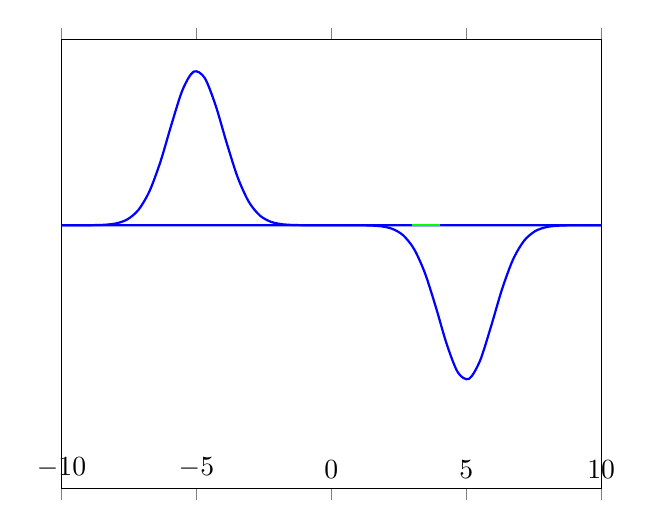
\begin{tikzpicture}
\begin{axis}[
    ymin=0.5,
    ymax=-0.5,
    xmin=-10,
    xmax=10,
    samples=50,
    domain=-10:10,
]
\addplot[blue, thick, smooth] {-1/(2*pi)^(1/2) * exp(-(x+5)^2/(2))};
    

\addplot[green, thick, fill=green!30, fill opacity=0.5,
    domain={3:4},
    restrict y to domain=-1:0,
    samples=50,
    ] {ifthenelse((3 < x) && (x < 4), -1/(2*pi)^(1/2) * exp(-(x+5)^2/2), 0)};
    
 \addplot[blue, thick, smooth] {1/(2*pi)^(1/2) * exp(-(x-5)^2/(2))};
\end{axis}
\end{tikzpicture}
\end{frame}
\end{comment}

%%%%%%%%%%%%%%%%%%%%%%%%%%%



%研究内容
\section{最適輸送問題の定式化}
\begin{frame}{最適輸送問題の定式化}
    \begin{block}{}
        $\Omega  \subset \mathbb{R}^d: \text{凸集合}$,\\
        $c: \Omega \times \Omega \to \mathbb{R}, \quad c(x, y) : x \text{から$y$への輸送にかかるコスト}$, \\
        $\mu, \nu : \Omega \text{上の確率測度},$\\
        $T: \Omega \to \Omega, \quad T_\#\mu = \nu: \text{$\mu$ を $\nu$ に運ぶ写像},$
        \vspace{\baselineskip} 

        $\mu$を$\nu$に移動させる最小コストを$C$とすると,最適輸送問題は以下のように定義される,
        \begin{equation*}
            C(\mu, \nu) = \inf_T \int_\Omega c(x, T(x)) d \mu (x).
        \end{equation*}

    \end{block}
\end{frame}

%カントロヴィッチ双対問題
\section{カントロヴィッチ双対問題}
\begin{frame}{カントロヴィッチ双対問題}
    \begin{block}{カントロヴィッチ双対問題}
        $\nu, \mu$: 確率測度, \quad
        $c(x, y) : x \text{から$y$への輸送にかかるコスト}$,\\
        \vspace{\baselineskip} 
        最適なコスト$C$は輸送する砂の体積を最大化させる問題として扱うことができる.
        \begin{equation*}
            C = \sup_{\phi, \psi} \int \phi  d\nu + \int \psi  d\mu 
        \end{equation*}

        ただし,Kantorovichポテンシャル$\phi(y), \psi(x)$は, 
    
        \begin{equation*}
            \phi(y) + \psi(x) \le c(x, y).
        \end{equation*}
    \end{block}
    $\mu \to \nu$への最適マップが存在すると、双対問題の最大値 $\phi_*(y), \psi_*(x)$が復元できる.

    そのとき, 
    \begin{equation*}
        \phi_*(y) + \psi_*(x) = c(x, y).
    \end{equation*}

\end{frame}

%c transform
\section{C変換}

\begin{frame}{c-変換}
    \begin{definition}[c-変換]

        連続関数 $\phi: \Omega \to \mathbb{R}$に対し, そのc-変換 $\phi^c: \Omega \to \mathbb{R}$を次のように定義する.
        \begin{equation*}
            \phi^c(x) := \inf_{y \in \Omega} \{ c(x, y) - \phi(y) \}
        \end{equation*}

        また, $\phi$ が c-凹関数とは, $\phi = \psi^c$ となる連続関数$\psi: \Omega \to \mathbb{R}$ が存在することをいう.

        さらに関数の組 $(\phi, \psi)$が c-共役であるとは, $\phi = \psi^c$ かつ $\psi = \phi^c$のときをいう.

    \end{definition}
    $(\phi, \psi)$が c-共役のとき, $\phi (y), \psi (x)$ の 最大値 $\phi_*, \psi_*$  は,
    \begin{equation*}
        \phi_*(y) = \psi_*^c(y) = \inf\{c(x, y) - \psi_*(x) \}
    \end{equation*}
    \begin{equation*}
        \psi_*(x) = \phi_*^c(x) = \inf\{c(x, y) - \phi_*(y) \}
    \end{equation*}
\end{frame}



\begin{frame}{The back-and-forth method(Matt Jacobs, Flavien Léger 2020)}
    カントロヴィッチ双対問題
    $C = \sup_{\phi, \psi} \int \phi  d\nu + \int \psi  d\mu $
    はc-変換を用いて,
    \begin{align*}
        J(\phi) &= \int \phi  d \nu + \int \phi^c  d \mu, &
        I(\psi) = \int \psi^c  d \nu + \int \psi  d \mu, 
    \end{align*}

    の$\sup$と表すことができる.\\
    \vspace{\baselineskip}
    $J$と$I$それぞれで勾配上昇法によって最大値を求め,$J$と$I$をc-変換で行き来することで,高速にカントロヴィッチ双対問題(最適輸送問題)を解くことができる.\\
    
    \begin{equation*}
        \huge J(\phi) \xrightleftharpoons[\psi^c = \phi]{\phi^c = \psi} I(\psi)
    \end{equation*}
    


\end{frame}


\begin{comment}

\section{pushforward}
\begin{frame}{押し出し測度}
    \begin{definition}[押し出し測度(pushforward measure)]
        $\mu$ から $\nu$ へ輸送する写像を$T$とするとき$(T_\#\mu = \nu)$,
        押し出し測度は
        \begin{equation*}
            T_\#\mu (A) := \mu (T^{-1} (A)) \qquad A \subset \Omega
        \end{equation*}
        で定義される.

        \vspace{\baselineskip} 

        $\Omega$ 上の確率測度$\mu, \nu$ がルベーグ測度において絶対連続とすると,
        $(T_\#\mu = \nu)$という制約条件下で,
        pushforwardは,任意の連続関数 $\phi$に対し,
        \begin{equation*}
            \int_\Omega \phi (T(x)) d \mu (x) = \int_\Omega \phi(y) d \nu (y).
        \end{equation*}
        と定義される.

    \end{definition}
\end{frame}

\begin{frame}{カントロヴィッチ双対問題の導入}

        \begin{align*}
            J(\mu, \nu) &= \inf_{T_\# \mu} \int_\Omega c(x, T(x)) d \mu (x)\\
                        &= \inf_{T_\# \mu} \sup_\phi \int_\Omega c(x, T(x)) d \mu (x) - \phi (T(x)) d \mu (x) + \int_\Omega \phi (y) d \nu (y)\\
                        \intertext{$\nu$は絶対連続より, infimum と supremum の入れ替え可能であるので,}
                        &= \sup_\phi \left( \inf_{T_\# \mu} \int_\Omega c(x, T(x)) d \mu (x) - \phi (T(x)) d \mu (x) + \int_\Omega \phi (y) d \nu (y) \right)\\
                        &= \sup_\phi \left( \int_\Omega \phi^c (x) d \mu (x) + \int_\Omega \phi (y) d \nu (y) \right)\\
                        &= \sup_\phi \left( \int_\Omega \phi^c d \mu + \int_\Omega \phi d \nu \right)\\
        \end{align*}

\end{frame} 

\end{comment}


% ブロック環境




%Algorithm
\section{Algorithm}
\begin{frame}{Algorithm}
    \begin{block}{Algorithm: the back-and-forth method}
        \begin{align*}
            \phi_{n + \frac{1}{2}} &= \phi_{n} + \sigma \nabla_{\dot{H}^1} J(\phi_{n}),\\
            \psi_{n + \frac{1}{2}} &= (\phi_{n + \frac{1}{2}})^c,\\
            \psi_{n + 1} &= \psi_{n + \frac{1}{2}} + \sigma \nabla_{\dot{H}^1} I(\psi_{n + \frac{1}{2}}),\\
            \phi_{n + 1} &= (\psi_{n + 1})^c.
        \end{align*}
    \end{block}

    \begin{enumerate}
        \item 勾配上昇法を以下条件のもとに行う.
        \begin{align*}
            \nabla_{\dot{H}^1} J(\phi) = (- \Delta)^{-1} (\nu - T_{\phi \#} \mu)\\
            \nabla_{\dot{H}^1} I(\psi) = (- \Delta)^{-1} (\mu - T_{\psi \#} \nu)\\
        \end{align*}
        \item back-and-forth methodで $J$ と $I$ で勾配上昇を交互に行う
    \end{enumerate}

\end{frame}

%Example 1
\section{Example 1: Update $\mu$ and $\nu$}
\begin{frame}{Example 1: Update $\mu$ and $\nu$}
    \begin{figure}[htb]
        \begin{center}
            \begin{minipage}{0.45\hsize}
                \includegraphics[width=\linewidth]{image/back-and-forth-update_ex1_0.png}
            \end{minipage}
            \begin{minipage}{0.45\hsize}
                \includegraphics[width=\linewidth]{image/back-and-forth-update_ex1_19.png}
            \end{minipage}
        \end{center}
    \end{figure}
    \label{Example 1}

    初期条件
    \begin{center}
    $\mu = \left\{
        \begin{array}{ll}
            1 & 0.3 \le x \le 0.8 \\
            0 & otherwise \\
        \end{array}
    \right.
    $
    $\nu = \left\{
        \begin{array}{ll}
            1 & - 0.8 \le x \le - 0.3 \\
            0 & otherwise \\
        \end{array}
    \right.
    $
    \end{center}

\end{frame}

%Example 2
\section{Example 2: Update $\mu$ and $\nu$}
\begin{frame}{Example 2: Update $\mu$ and $\nu$}
    \begin{figure}[htb]
        \begin{center}
            \begin{minipage}{0.45\hsize}
                \includegraphics[width=\linewidth]{image/back-and-forth-update_ex2_0.png}
            \end{minipage}
            \begin{minipage}{0.45\hsize}
                \includegraphics[width=\linewidth]{image/back-and-forth-update_ex2_19.png}
            \end{minipage}
        \end{center}
    \end{figure}
    \label{Example 2}

    初期条件
    \begin{center}
    $\mu = \left\{
        \begin{array}{ll}
            0.5 & 0 \le x \le 0.5 \\
            0 & otherwise \\
        \end{array}
    \right.
    $
    $\nu = \left\{
        \begin{array}{ll}
            1 & - 0.5 \le x \le - 0.25 \\
            0 & otherwise \\
        \end{array}
    \right.
    $
    \end{center}

\end{frame}

\section{問題点}
\begin{frame}{問題点}

    \begin{block}{transport map}
        $T_{\phi \#} \mu = \nu, T_{\psi \#} \nu = \mu$
    \end{block}

    \begin{figure}[htb]
        \begin{center}
            \begin{minipage}{0.40\hsize}
                \includegraphics[width=\linewidth]{image/x[iopt]explanation1.JPG}
            \end{minipage}
            \begin{minipage}{0.40\hsize}
                \includegraphics[width=\linewidth]{image/x[iopt]explanation2.JPG}
            \end{minipage}
        \end{center}
    \end{figure}
    \label{x[iopt]explanation}

    transport前と後の$x$座標が一対一対応であるため,

    ある$x$での$\nu$と$\mu$の質量(値)がそのままtransport先へ反映される.

\end{frame}

\section{今後}
\begin{frame}{今後}
    \begin{itemize}
        \item 一対一対応ではないtransport mapのプログラム作成(精度向上のため)
        \item back and forth methodを用いて偏微分方程式を解くプログラムの作成
        \item 特に非線型方程式の新しい解法を求めるプログラムを作成
    \end{itemize}

\end{frame}

\section{参考文献}
\begin{frame}{参考文献}
    \begin{thebibliography}{3}
        \bibitem{1}
        Matt Jacobs, Flavien Léger.
        \newblock A fast approach to optimal transport: the back-and-forth method.
        \newblock Numerische Mathematik, 2020. 
        \bibitem{2}
        太田 慎一.
        \newblock 最適輸送理論とその周辺.
        \newblock \url{http://www4.math.sci.osaka-u.ac.jp/~sohta/jarts/kino09.pdf}
        \bibitem{3}
        小林 愼一郎.
        \newblock 距離コストに対する最適輸送問題について.
        \newblock \url{https://www.math.sci.hokudai.ac.jp/~wakate/mcyr/2020/pdf/kobayashi_shinichiro.pdf}.
    \end{thebibliography}
\end{frame}

\begin{comment}
\section{箇条書き}
\begin{frame}{箇条書き}
    \begin{itemize}
        \item item 1
        \begin{enumerate}
            \item item1-1
            \item item1-2
        \end{enumerate}
        \item item 2
        \begin{enumerate}[I]
            \item item 2-1
            \item item 2-2
            \item item 2-3
        \end{enumerate}
    \end{itemize}
\end{frame}




% 数学ブロック環境
\begin{frame}{数学ブロック環境}
\begin{theorem}[定理名] 
$e^{ix} = \cos x + i \sin x$
\end{theorem}
\begin{definition}[定義名]
$e^{x} \approx 1 + x$
\end{definition}
\begin{corollary}[系名]
$a + b + c = 0$
\end{corollary}
\begin{proof}
$\int_{-\infty}^{\infty} e^{-a x^{2}} = 2 \int_{0}^{\infty} e^{-a x^{2}}$
\end{proof}
\end{frame}

% 表スライド
\section{表}
\begin{frame}{表の追加}
    \begin{table}
        \caption{Caption}
        \label{table:sample}
        \centering
            \begin{tabular}{ccc}
            \hline
            料理    & 値段   &  場所  \\
            \hline \hline
            チキン  & 200円  & 公園 \\
            ピザ    & 300円  & 公園 \\
            ご飯    & 100円  & 室内 \\
            パン    &  70円  &  室内 \\
            \hline
            \end{tabular}
    \end{table}
\end{frame}
\end{comment}
\end{document}




